\documentclass[12pt,a4paper]{article}
\usepackage{pgf}
% \usepackage[condensed,math]{kurier}
% \usepackage[T1]{fontenc}
\usepackage{svg}
\usepackage{tikz}
\usepackage{stanli}
\usepackage{afterpage}
\usepackage{multirow}
\usepackage{subfig}
\usepackage{pgfpages}
\usepackage{svg}
\usepackage{rotating}
\usepackage[utf8]{inputenc}
\usepackage{enumitem}
\usepackage[a4paper, top=1in, bottom=1in, left=1in, right=1in]{geometry}
\usepackage{geometry}
\usepackage{array}
\usepackage{enumitem}
\usepackage{boldline}
\usepackage{pdflscape} % Required for landscape pages
\usepackage{geometry}
\usepackage{setspace}
\usepackage{graphicx} % Required for inserting images
\usepackage{svg} % Required for inserting images in svg format
\usepackage{listings}
\usepackage{xcolor}
\usepackage[hidelinks]{hyperref}

% Definizione del colore blu per le parole chiave
\definecolor{keywords}{RGB}{0,0,255}

\lstset{
    language=SQL,
    basicstyle=\ttfamily,
    keywordstyle=[1]\color{keywords},  % Colore per le parole chiave di tipo 1
    morekeywords=[1]{IF, EXISTS, DATE_ADD, boolean},     % Aggiunta di parole chiave di tipo 1
}

\geometry{a4paper, margin=1in}
\setlist{noitemsep}

\renewcommand{\contentsname}{Indice} %cambiare nome alla table of content

%\usepackage{times}


\pgfpagesdeclarelayout{boxed}
{
	\edef\pgfpageoptionborder{0pt}
}
{
	\pgfpagesphysicalpageoptions
	{%
		logical pages=1,%
	}
	\pgfpageslogicalpageoptions{1}
	{
		border code=\pgfsetlinewidth{2pt}\color{black}\pgfstroke,%
		border shrink=\pgfpageoptionborder,%
		resized width=.9\pgfphysicalwidth,%
		resized height=.9\pgfphysicalheight,%
		center=\pgfpoint{.5\pgfphysicalwidth}{.5\pgfphysicalheight}%
	}%
}

%\pgfpagesuselayout{boxed}

\begin{document}

\begin{titlepage}

\newcommand{\HRule}{\rule{\linewidth}{0.5mm}} % Defines a new command for the horizontal lines, change thickness here

\center % Center everything on the page
 
%----------------------------------------------------------------------------------------
%	HEADING SECTIONS
%----------------------------------------------------------------------------------------

\textsc{\LARGE Università degli Studi di Torino}\\[1.5cm] % Name of your university/college

\includegraphics[scale=.1]{unito informatica.jpg}\\[1cm] % Include a department/university logo - this will require the graphicx package
\textsc{\Large Basi di Dati}\\[0.5cm] % Major heading such as course name
\textsc{\large MFN0602}\\[0.5cm] % Minor heading such as course title

%----------------------------------------------------------------------------------------
%	TITLE SECTION
%----------------------------------------------------------------------------------------

\HRule \\[0.4cm]
{ \huge \bfseries Progetto}\\[0.4cm] % Title of your document
\HRule \\[1.5cm]
 
%----------------------------------------------------------------------------------------
%	AUTHOR SECTION
%----------------------------------------------------------------------------------------

\begin{minipage}{0.4\textwidth}
\begin{center} \large
Oskar Heise\\ % Your name
\end{center}

\end{minipage}\\[2cm]

% If you don't want a supervisor, uncomment the two lines below and remove the section above
%\Large \emph{Author:}\\
%John \textsc{Smith}\\[3cm] % Your name

%----------------------------------------------------------------------------------------
%	DATE SECTION
%----------------------------------------------------------------------------------------

{\large 2022/2023}\\[2cm] % Date, change the \today to a set date if you want to be precise

\vfill % Fill the rest of the page with whitespace
\end{titlepage}

\newpage
\tableofcontents
\newpage


\newgeometry{margin=1.8cm}
\section{Progettazione Concettuale}
\subsection{Requisiti iniziali}
Si vuole realizzare una base di dati per un servizio che permette di fare live streaming su vari
argomenti. Il live streaming (o, più sinteticamente, la live) permette di interagire con il pubblico in
tempo reale grazie a feed video, chat e altro.
Ogni utente può essere spettatore o streamer, o entrambi. Gli spettatori possono essere registrati
al servizio oppure possono guardare le live in modo anonimo. Per registrarsi, gli utenti devono
indicare nome utente, password, data di nascita, numero di telefono o indirizzo mail. Gli utenti
iscritti possono chattare, seguire lo streamer, creare dirette.
Gli streamer hanno ciascuno un canale, che può essere caratterizzato tramite una descrizione. Per
ogni canale, è possibile specificare una lista di social associati (ad esempio Instagram, YouTube,
ecc.), un’immagine profilo e anche un trailer (Figura 1(a)). In ogni canale possono esserci live,
video (live passate) e clip (video di durata breve). Le live possono anche non diventare video del
canale. Ognuno ha un titolo, una durata, appartiene a una categoria (Figura 1(b)) e può essere
associato a diversi tag. Per ogni live viene memorizzato il numero medio di spettatori mentre per i
video e le clip il numero di visualizzazioni.

\begin{figure}[h]
    \centering
    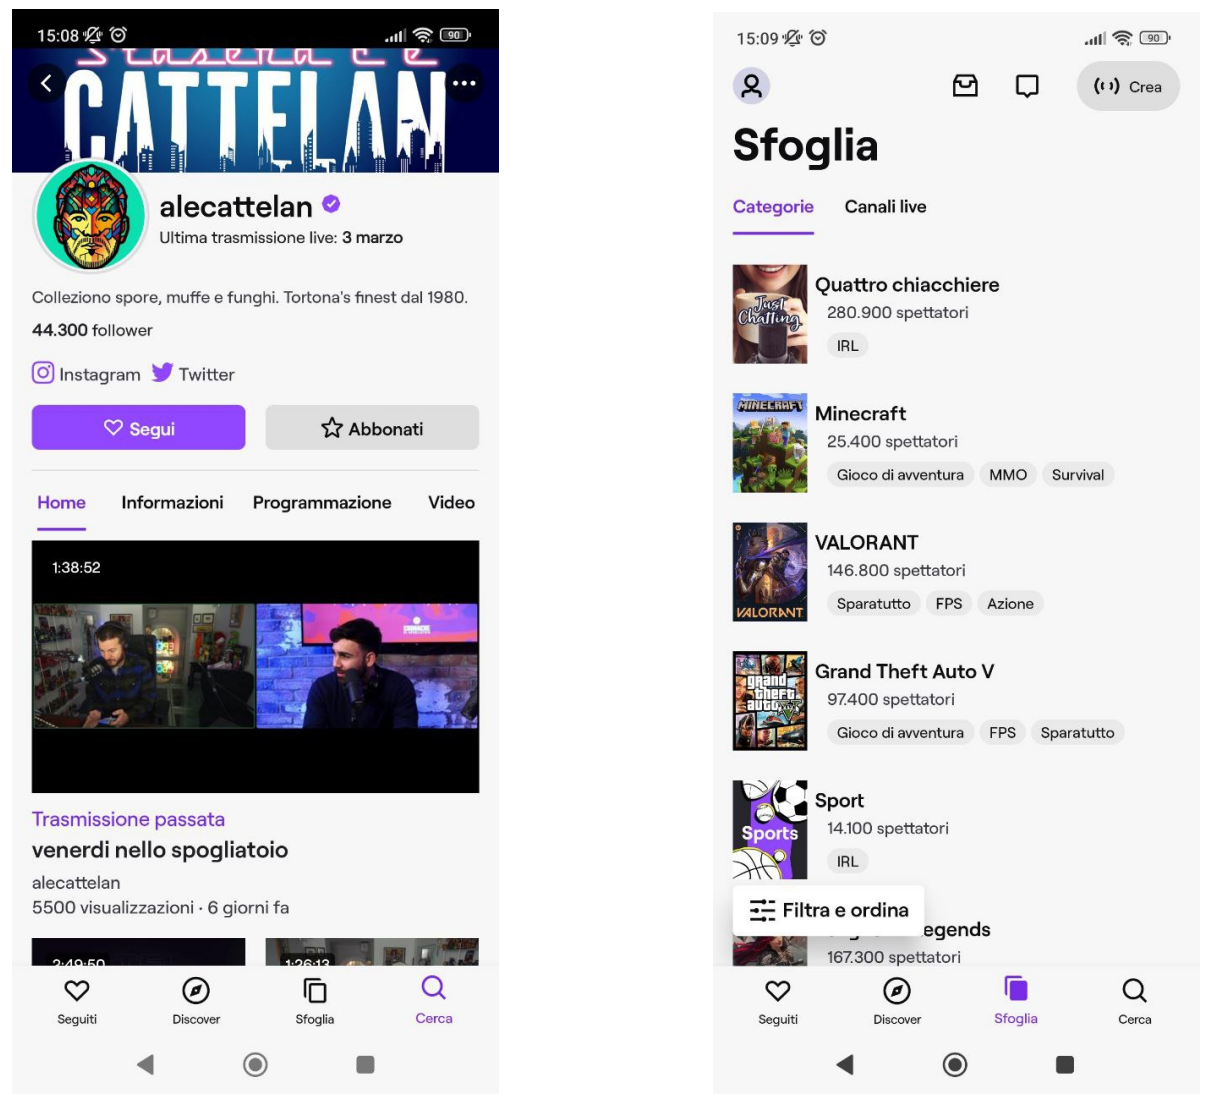
\includegraphics[width=0.5\linewidth]{img/twitch.png}
\end{figure}

Per ogni creatore di contenuti, si memorizzano il numero di live effettuate, il numero di minuti
trasmessi, il numero medio di spettatori simultanei. Inoltre, sulla pagina del canale viene
visualizzato il numero di follower.
Quando uno streamer rispetta determinati parametri di performance (un minimo di 500 minuti
trasmessi, una media di tre o più spettatori simultanei, almeno 50 follower), può diventare affiliate.
Le stream hanno degli orari. Ogni streamer ha un calendario in cui può dire quando farà stream e
indicare il titolo delle prossime live.
I viewer possono diventare follower del canale degli streamer che preferiscono, e le loro
preferenze sono raccolte in un elenco di follower a cui possono accedere dal loro profilo. I viewer
possono inoltre supportare gli streamer tramite la subscription (a pagamento) al loro canale,
ottenendo dei privilegi (emoticon personalizzate, ecc.). Inoltre, gli utenti hanno un portafoglio di bit
(moneta virtuale che possono acquistare tramite la piattaforma), che possono usare per fare
donazioni agli streamer.
Oltre a chattare pubblicamente, gli utenti possono scambiarsi messaggi privati.

La base di dati deve supportare le seguenti operazioni:
\begin{itemize}
    \item Una volta al giorno si controllano le condizioni per la qualifica di affiliate.
    \item Una volta a settimana viene calcolata la classifica degli streamer più seguiti.
\end{itemize}
Si può assumere che i contenuti multimediali vengano gestiti da una piattaforma di video hosting e
che quindi sia sufficiente memorizzare un URL.
\restoregeometry



\newgeometry{margin=0.5cm}
\begin{landscape}
\setlength{\parskip}{2em}
\subsection{Glossario dei termini}
\begin{center}
\begin{tabular}{ |p{5cm}|p{7cm}|p{4cm}|p{5cm}|  }
 \hline
 \multicolumn{1}{|c|}{\textbf{Termine}} 
 & \multicolumn{1}{|c|}{\textbf{Descrizione}} 
 & \multicolumn{1}{|c|}{\textbf{Sinonimi}}
 & \multicolumn{1}{|c|}{\textbf{Collegamenti}}\\
 \hline
 Utente & Partecipante della piattaforma & Pubblico & Calendario, Portafoglio bit, Chat pubblica, Chat privata, Canale, Subscription, Donazione\\
 \hline
 Content creator & Creatore di contenuti & Streamer, Creatore di contenuti & Contenuti\\
 \hline
 Affiliato & Partner Twitch & N.D. & Donazione, Subscription\\
 \hline
 Portafoglio bit & Borsellino virtuale di bit & Wallet & Utente\\
 \hline
 VOD & Video on Demand & N.D. & N.D.\\
 \hline
 Clip & Momenti salienti di un VOD & Video di breve durata & N.D.\\
 \hline
 Video & Contenuto video & Live passata & N.D.\\
 \hline
 Contenuti & Materiale contenutistico & N.D. & Content Creator\\
 \hline
 Live streaming & Trasmissione in diretta & Live, Stream & Utente anonimo, Chat pubblica, Content creator\\
 \hline
 Calendario & Programma settimanale & N.D. & Live streaming, Utente\\
 \hline
 Utente anonimo & Anonimo & Viewer & Live streaming\\
 \hline 
 Chat pubblica & Chatroom globale & Chat & Utente, Live streaming\\
 \hline
 Chat privata & Conversazione privata & Chat & Utente\\
 \hline
 Canale & Profilo utente & N.D. & Utente\\
 \hline 
 Subscription & Iscrizione & N.D. & Utente,  Affiliato\\
 \hline
 Donazione & Contributo monetario & N.D. & Utente, Affiliato\\
 \hline
\end{tabular}
\end{center}
\end{landscape}
\restoregeometry

\subsection{Requisiti rivisti e strutturati in frasi omogenee}
\begin{itemize}
    \item La piattaforma per la quale si vuole realizzare una base di dati è destinata ad ospitare contenuti multimediali, in particolare live streaming, video e clip.
    Il live streaming permette di interagire con il pubblico in tempo reale grazie a feed video, chat e altro.
    \item Ogni utente può essere spettatore o streamer, o entrambi. Per registrarsi, gli utenti devono indicare nome utente, password, data di nascita, numero di telefono o indirizzo mail. Gli utenti registrati possono chattare, seguire lo streamer, creare live streaming.
    \item Gli spettatori possono essere registrati al servizio oppure possono guardare le live streaming in modo anonimo. Gli spettatori registrati possono diventare follower del canale degli streamer che preferiscono e le loro preferenze sono raccolte in un elenco di followee a cui possono accedere dal loro profilo. Gli spettatori possono inoltre supportare gli streamer tramite la subscription (a pagamento) al loro canale, ottenendo dei privilegi (emoticon personalizzate, ecc.). Inoltre, gli utenti hanno un portafoglio di bit (moneta virtuale che possono acquistare tramite la piattaforma), che possono usare per fare donazioni agli streamer.
    Oltre a chattare pubblicamente, gli utenti registrati possono scambiarsi messaggi privati.
    \item Per ogni streamer si memorizzano il numero di live streaming effettuate, il numero di minuti trasmessi, il numero di medio di spettatori simultanei. 
    Quando uno streamer rispetta determinati parametri di performance (un minimo di 500 minuti trasmessi, una media di tre o più spettatori simultanei, almeno 50 follower), può diventare \textit{affiliate}.
    Ogni streamer ha un calendario in cui può dire quando farà stream e indicare il titolo delle prossime live streaming. 
    \item Gli streamer hanno ciascuno un canale, che può essere caratterizzato tramite una descrizione. In ogni canale possono esserci live streaming, video (live streaming passate) e clip (video di durata breve). Ognuno ha un titolo, una durata, appartiene a una categoria e può essere associato a diversi tag. Per ogni live streaming viene memorizzato il numero medio di spettatori mentre per i video e le clip il numero di visualizzazioni. Le live streaming possono anche non diventare video del canale. Si può assumere che i contenuti multimediali vengano gestiti da una piattaforma di video hosting e che quindi sia sufficiente memorizzare un URL.
\end{itemize}

\newpage
\newgeometry{margin=0.5cm}
\begin{landscape}
\subsection{Schema E-R principale + business rules}
\vspace{-\parskip} % Elimina lo spazio aggiunto dall'intestazione della subsection
\subsubsection{Schema E-R}
\vspace{-\parskip} % Elimina lo spazio aggiunto dall'intestazione della subsection
\begin{figure}[h]
    \centering
    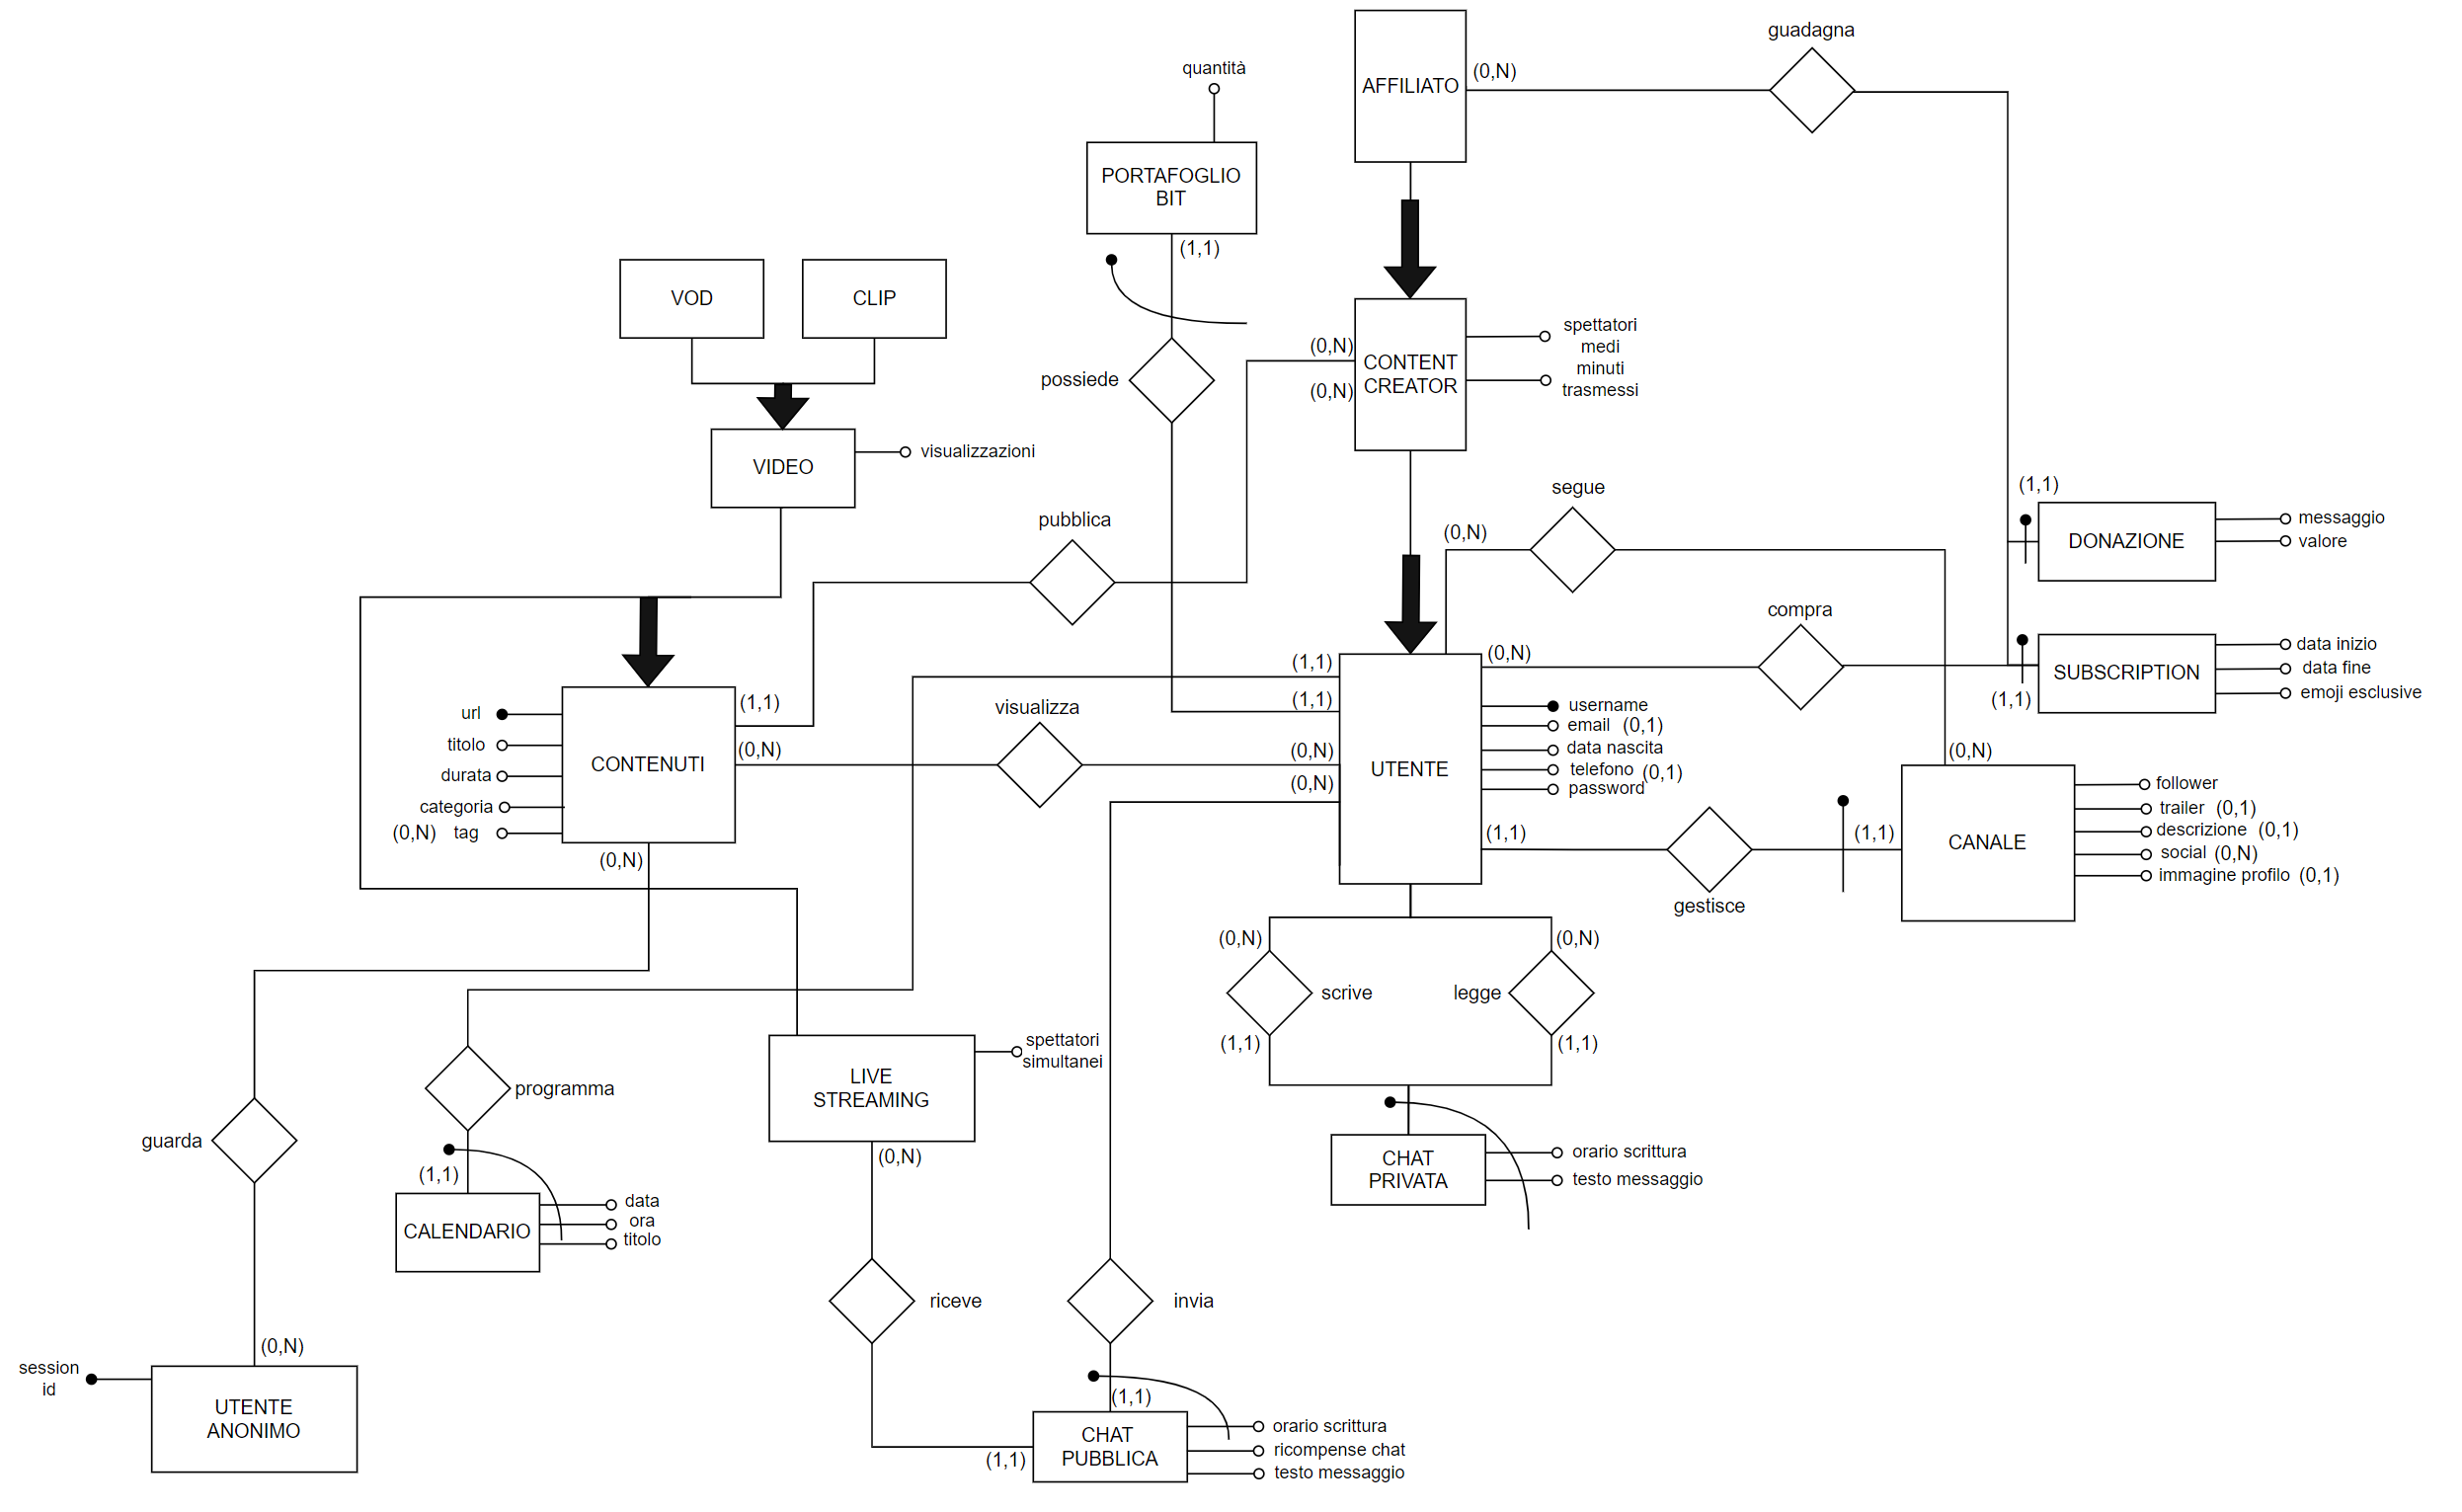
\includegraphics[scale=0.5]{img/ER1.png}
\end{figure}
\end{landscape}
\restoregeometry


\newpage
\setlength{\parskip}{0.5em}
\newgeometry{margin=0.5cm}
\begin{landscape}
\subsubsection{Business Rules}
\subsubsection*{Dizionario dei dati per le entità}
\begin{center}
\begin{tabular}{ |p{5cm}|p{4cm}|p{7cm}|p{5cm}|  }
 \hline
 \multicolumn{1}{|c|}{\textbf{Entità}} 
 & \multicolumn{1}{|c|}{\textbf{Descrizione}} 
 & \multicolumn{1}{|c|}{\textbf{Attributi}}
 & \multicolumn{1}{|c|}{\textbf{Identificatore}}\\
 \hline
 Utente & Partecipante della piattaforma & Username, Email, Data di nascita, Telefono, Password & Username\\
 \hline
 Content creator & Creatore di contenuti & Username, Email, Data di nascita, Telefono, Password, Spettatori medi, Minuti trasmessi & Username \\
 \hline
 Affiliato & Partner Twitch & Username, Email, Data di nascita, Telefono, Password, Spettatori medi, Minuti trasmessi & Username\\
 \hline
 Portafoglio bit & Borsellino virtuale di bit & Quantità & Username\\
 \hline
 Contenuti & Materiale contenutistico & URL, Titolo, Durata, Categoria, Tag & URL \\
 \hline
  Video & Contenuto video & URL, Visualizzazioni, Titolo, Durata, Categoria, Tag & URL \\
 \hline
 VOD & Video on Demand & URL, Visualizzazioni, Titolo, Durata, Categoria, Tag & URL \\
 \hline
 Clip & Momenti salienti di una diretta & URL, Visualizzazioni, Titolo, Durata, Categoria, Tag & URL\\
 \hline
 Live streaming & Trasmissione in diretta & URL, Spettatori simultanei, Titolo, Durata, Categoria, Tag & URL \\
 \hline
 Calendario & Programma settimanale & Data, Ora, Titolo & Data, Ora\\
 \hline
 Utente anonimo & Anonimo & Session id & Session id\\
 \hline 
 Chat pubblica & Chatroom globale & Orario scrittura, Ricompense chat, Testo messaggio & Username, Orario scrittura\\
 \hline
 Chat privata & Conversazione privata & Orario scrittura, Testo messaggio & Username, Orario scrittura, Testo messaggio\\
 \hline
 Canale & Profilo utente & Follower, Trailer, Descrizione, Social, Immagine profilo & Username\\
 \hline 
 Subscription & Iscrizione & Data inizio, Data fine, Emoji esclusive & Username\\
 \hline
 Donazione & Contributo monetario & Messaggio, Valore & Username\\
 \hline
\end{tabular}
\end{center}
\end{landscape}
\restoregeometry








\newpage
\setlength{\parskip}{0.5em}
\newgeometry{margin=0.5cm}
\begin{landscape}
\subsubsection*{Dizionario dei dati per le relazioni}
\begin{center}
\begin{tabular}{ |p{5cm}|p{4cm}|p{7cm}|p{2cm}|  }
 \hline
 \multicolumn{1}{|c|}{\textbf{Relazione}} 
 & \multicolumn{1}{|c|}{\textbf{Descrizione}} 
 & \multicolumn{1}{|c|}{\textbf{Componenti}}
 & \multicolumn{1}{|c|}{\textbf{Attributi}}\\
 \hline
 Possiede & Possesso di un portafoglio di bit & Utente (1,1), Portafoglio bit (1,1) & N.D.\\
 \hline
 Pubblica & Pubblicazione di contenuti & Contenuti (1,1), Content creator (0,N) & N.D. \\
 \hline
 Programma & Invio di un evento nel calendario & Calendario (1,1), Utente (1,1) & N.D.\\
 \hline
 Guarda & Visualizzazione di una diretta da utente anonimo & Utente anonimo (0,N), Contenuti (0,N) & N.D.\\
 \hline
 Visualizza & Visualizzazione di una diretta da utente registrato & Contenuti (O,N), Utente (0,N) & N.D. \\
 \hline
 Riceve & Ricezione di un messaggio pubblico & Live streaming (0,N), Chat pubblica (1,1) & N.D.\\
 \hline
 Invia & Invio di un messaggio pubblico & Utente (0,N), Chat pubblica (1,1) & N.D.\\
 \hline
 Scrive & Scrittura di un messaggio privato & Utente (0,N), Chat privata (1,1) & N.D.\\
 \hline
 Legge & Lettura di un messaggio privato & Chat privata (1,1), Utente (0,N) & N.D.\\
 \hline
 Gestisce & Gestione e possesso di un canale & Utente (1,1), Canale (1,1) & N.D.\\
 \hline
 Compra & Acquisto di una subscription o donazione & Donazione (1,1), Subscription (1,1), Utente (0,N) & N.D.\\
 \hline
 Guadagna & Guadagno di una donazione o di una Subscription & Donazione (1,1), Subscription (1,1), Affiliato (0,N) & N.D.\\
 \hline
 Segue & Follow di un utente verso un canale & Utente (0,N), Canale (0,N) & N.D.\\
 \hline
\end{tabular}
\end{center}
\end{landscape}
\restoregeometry















\subsubsection{Vincoli di Integrità}
\setlength{\parskip}{0.5em}

\begin{itemize}
\item \textbf{Utente:}
  \begin{itemize}
    \item Deve avere un nome utente univoco.
    \item Può seguire altri utenti per ricevere notifiche.
  \end{itemize}

\item \textbf{Content Creator:}
  \begin{itemize}
    \item Può guadagnare denaro tramite pubblicità e abbonamenti.
    \item Deve seguire le linee guida di Twitch.
  \end{itemize}

\item \textbf{Affiliato:}
  \begin{itemize}
    \item Deve rispettare gli accordi di partnership con Twitch.
    \item Può guadagnare una percentuale sui ricavi pubblicitari.
    \item Deve pubblicare contenuti originali.
  \end{itemize}

\item \textbf{Contenuti:}
  \begin{itemize}
    \item I contenuti non devono violare i diritti d'autore.
    \item Devono rispettare le linee guida di Twitch.
  \end{itemize}

\item \textbf{Chat Pubblica:}
  \begin{itemize}
    \item La chat pubblica non deve contenere linguaggio offensivo o contenuti inappropriati.
  \end{itemize}

\item \textbf{Chat Privata:}
  \begin{itemize}
    \item Le chat private non devono essere utilizzate per scopi illegali o dannosi.
  \end{itemize}

\item \textbf{Subscription:}
  \begin{itemize}
    \item Le iscrizioni devono essere ottenute onestamente.
  \end{itemize}

\item \textbf{Donazione:}
  \begin{itemize}
    \item Non si può effettuare una donazione se il portafoglio non contiene bits.
  \end{itemize}
\end{itemize}


\newpage
\section{Progettazione Logica}
\subsection{Tavola dei volumi}
Si stima una quantità di risorse partendo da un numero di utenti pari a 5 milioni. \\
\textbf{Nota Bene} \ \ E: Entità R: Relazione 
\subsection{Tavola dei volumi}
\begin{center}
\begin{tabular}{ |p{5cm}|p{2cm}|p{4cm}|  }
 \hline
 \multicolumn{1}{|c|}{\textbf{Concetto}} 
 & \multicolumn{1}{|c|}{\textbf{Tipo}} 
 & \multicolumn{1}{|c|}{\textbf{Volume}}\\
  \hline
 Utente & E & 5.000.000\\
  \hline
 Content creator & E & 500.000\\
 \hline 
  Affiliato & E & 400.000\\
 \hline
 Portafoglio bit & E & 5.000.000\\
 \hline
 Contenuti & E & 260.000.000\\
 \hline
  Video & E & 208.000.000\\
 \hline
 VOD & E & 52.000.000\\
 \hline
 Clip & E & 156.000.000\\
 \hline
 Live streaming & E & 52.000.000\\
 \hline
 Calendario & E & 5.000.000\\
 \hline 
  Utente anonimo & E & 200.000\\
 \hline
 Chat pubblica & E & 20.000.000.000\\
 \hline
 Chat privata & E & 25.000.000\\
 \hline
 Canale & E & 5.000.000\\
 \hline 
 Subscription & E & 4.000.000\\
 \hline
 Donazione & E & 18.750.000\\
 \hline
 Possiede & R & 5.000.000\\
 \hline
 Pubblica & R & 260.000.000\\
 \hline
 Programma & R & 5.000.000\\
 \hline
 Guarda & R & 2.400.000\\
 \hline
 Visualizza & R &  2.880.000.000\\
 \hline
 Riceve & R & 20.000.000.000\\
 \hline
 Invia & R & 20.000.000.000\\
 \hline
 Scrive & R & 25.000.000\\
 \hline
 Legge & R & 25.000.000\\
 \hline
 Gestisce & R & 5.000.000\\
 \hline
 Compra & R & 21.750.000\\
 \hline
 Guadagna & R & 21.750.000\\
 \hline
 Segue & R & 50.000.000\\
 \hline
\end{tabular}
\end{center}

\newpage
\subsection{Spiegazione dei dati}
\begin{itemize}
    \item \textbf{Utente:} Per semplificare l'analisi ed utilizzare volumi minori, si suppone che la piattaforma venga utilizzata da 5.000.000 di utenti.
    \item \textbf{Content creator:} Si suppone di avere 500.000 utenti che creano contenuti nella piattaforma.
    \item \textbf{Affiliato:} Suppongo che i content creator affiliati siano circa 400.000.
    \item \textbf{Portafoglio bit:} Ogni utente possiede un portafoglio bit.
    \item \textbf{Contenuti:} Si stima che i contenuti prodotti all'anno da ogni singolo streamer siano 520, ovvero 10 a settimana, di cui 2 dirette, 2 VOD e 6 Clip. Avrò quindi 260.000.000 di contenuti all'anno divisi secondo le stime fatte in precedenza.
    \item \textbf{Video:} Secondo i calcoli fatti in precedenza ho 208.000.000 all'anno.
    \item \textbf{VOD:} Secondo i calcoli fatti in precedenza 52.000.000 ho all'anno.
    \item \textbf{Clip:} Secondo i calcoli fatti in precedenza ho 156.000.000 all'anno.
    \item \textbf{Live streaming:} Secondo i calcoli fatti in precedenza ho 52.000.000 all'anno.
    \item \textbf{Calendario:} Ogni utente possiede un calendario.
    \item \textbf{Utente anonimo:} Si suppone che gli utenti anonimi siano solamente il 5\% degli utilizzatori della piattaforma.
    \item \textbf{Chat pubblica:} Si stima che ogni utente invii circa 80 messaggi pubblici a settimana.
    \item \textbf{Chat privata:} Si stima che ogni utente invii solamente 5 messaggi privati l'anno, visto che si tratta di una feature usata rarissimamente.
    \item \textbf{Canale:} Ogni utente possiede un canale.
    \item \textbf{Subscription:} Suppongo che il 50\% degli utenti sia disposto a supportare un content creator affiliato. Suppongo che in media ogni utente disposto ha più di un abbonamento all'attivo.
    \item \textbf{Donazione:} Le donazioni tendono ad essere più delle subscription. Suppongo che il 70\% degli utenti sia disposto a effettuare una donazione. Suppongo che ogni utente faccia circa 5 donazioni l'anno.
    \item \textbf{Possiede:} Ogni utente possiede uno e un solo portafoglio di bit.
    \item \textbf{Pubblica:} Il numero di pubblicazioni equivale al numero di contenuti presenti nella piattaforma, quindi 260.000.000.
    \item \textbf{Programma:} Ogni utente possiede uno e un solo calendario.
    \item \textbf{Guarda:} Stimo che vista l'assenza di un account, un utente anonimo guardi solamente 1 live al mese in media.
    \item \textbf{Visualizza:} Stimo che ogni utente registrato visualizzi in media 50 contenuti al mese, quindi tutti gli utenti guarderanno 2.880.000.000 contenuti l'anno.
    \item \textbf{Riceve:} Il numero è pari al numero di messaggi presenti nella chat pubblica durante le dirette.
    \item \textbf{Invia:} Il numero è pari al numero di messaggi inviati in media nella chat pubblica durante le dirette.
    \item \textbf{Scrive:} Il numero è pari al numero di messaggi inviati in media nella chat privata.
    \item \textbf{Legge:} Il numero è pari al numero di messaggi ricevuti in media nella chat privata.
    \item \textbf{Gestisce:} Ogni utente possiede uno e un solo canale.
    \item \textbf{Compra:} Seguendo il punto subscription e donazione spiegato in precedenza, all'anno vengono effettuati 4.000.000 + 18.750.000 acquisti.
    \item \textbf{Guadagna:} Il numero è lo stesso del punto precedente.
    \item \textbf{Segue:} Stimo che ogni utente segui in media altri 10 canali.
\end{itemize}







\newpage
\subsection{Tavola delle operazioni}
\begin{center}
\begin{tabular}{|p{10cm}|p{1cm}|p{3cm}|}
 \hline
 \multicolumn{1}{|c|}{\textbf{Operazione}} 
 & \multicolumn{1}{|c|}{\textbf{Tipo}}
 & \multicolumn{1}{|c|}{\textbf{Frequenza}}\\
  \hline
  Controllo delle condizioni per la qualifica di affiliato & I & 1/giorno\\
  \hline
  Calcolo della classifica degli streamer più seguiti & B & 1/settimana\\
 \hline
  Creazione di contenuti & I & 712.329/giorno\\
  \hline
  Visualizzazione dei contenuti & I & 7.896.986/giorno\\
 \hline 
  Invio messaggi in chat pubblica & I & 54.794.521/giorno\\
 \hline
  Scrittura messaggi in chat privata & I & 68.493/giorno\\
 \hline
  Follow di un utente verso un canale & I & 136.986/giorno\\
 \hline
\end{tabular}
\end{center}






\subsection{Ristrutturazione dello schema E-R}

\subsubsection{Analisi delle ridondanze}
Le ridondanze rilevate nel primo schema E-R sono le seguenti:
\begin{itemize}
\itemsep0.5em
    \item L'attributo \textit{Follower} presente nell'entità \textit{Canale} è ridondante poichè il numero di follower guadagnati da un content creator può essere incluso nella relazione \textit{Segue}.
    \item L'attributo \textit{Spettatori medi} presente nell'entità \textit{Content creator} è ridondante poichè il numero medio di spettatori di uno streamer può essere calcolato attraverso l'attributo \textit{Spettatori simultanei} presente nell'entità \textit{Live streaming}.
    \item L'attributo \textit{Minuti trasmessi} presente nell'entità \textit{Concent creator} è ridondante poichè il numero di minuti trasmessi può essere calcolato attraverso l'attributo \textit{Durata} presente nell'entità \textit{Contenuti}.
\end{itemize}



\subsubsection*{Analisi ridondanza \textit{Follower}}
\begin{figure}[h]
    \centering
    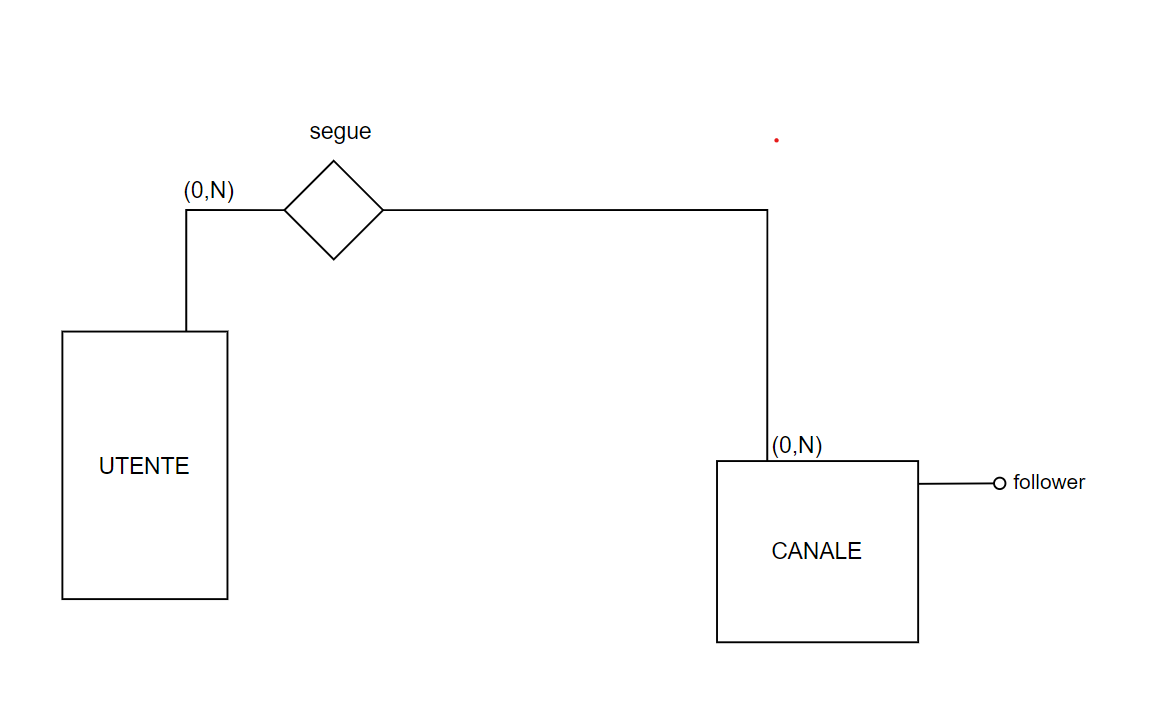
\includegraphics[scale = 0.5]{img/ridondanza1.png}
\end{figure}
\begin{center}
\begin{tabular}{|p{5cm}|p{5cm}|p{5cm}|}
\hline
\multicolumn{3}{|c|}{\textbf{Tavola dei volumi}}\\
\hline
 \multicolumn{1}{|c|}{\textbf{Concetto}} 
 & \multicolumn{1}{|c|}{\textbf{Tipo}}
 & \multicolumn{1}{|c|}{\textbf{Volume}}\\
  \hline
  Utente& E & 5.000.000\\
  \hline
  Canale & E & 5.000.000\\
 \hline 
  Segue & R & 50.000.000\\
 \hline
\end{tabular}
\end{center}
\begin{center}
\begin{tabular}{|p{5cm}|p{5cm}|p{5cm}|}
\hline
\multicolumn{3}{|c|}{\textbf{Tavola delle operazioni}}\\
\hline
 \multicolumn{1}{|c|}{\textbf{Operazone}} 
 & \multicolumn{1}{|c|}{\textbf{Tipo}}
 & \multicolumn{1}{|c|}{\textbf{Frequenza}}\\
  \hline
  Follow di un utente verso un canale & I & 136.986/giorno\\
  \hline
  Calcolo della classifica degli streamer più seguiti & B & 1/settimana\\
 \hline
\end{tabular}
\end{center}


\subsubsection*{Senza ridondanza} 
\textbf{Operazione 1:} Un utente inizia a seguire un altro utente, in media 136.986 volte al giorno.
\begin{figure}[h]
    \centering
    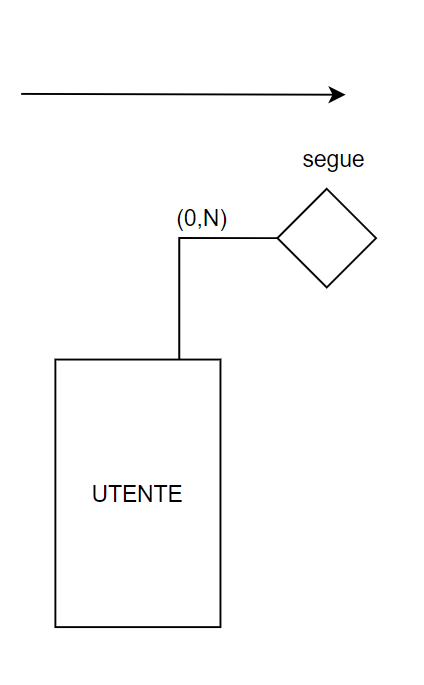
\includegraphics[scale = 0.5]{img/ridondanza11.png}
\end{figure}
\begin{center}
\begin{tabular}{|p{3cm}|p{3cm}|p{3cm}|p{3cm}|}
\hline
\multicolumn{4}{|c|}{\textbf{Tavola degli accessi}}\\
\hline
 \multicolumn{1}{|c|}{\textbf{Concetto}} 
 & \multicolumn{1}{|c|}{\textbf{Costrutto}}
 & \multicolumn{1}{|c|}{\textbf{Accessi}}
 & \multicolumn{1}{|c|}{\textbf{Tipo}}\\
  \hline
  Utente & E & 1 & S\\
  \hline
  Segue & R & 1 & S\\
 \hline
\end{tabular}
\end{center}
\paragraph{Nota Bene} S: Accesso in scrittura. \\ \\
\newpage
\textbf{Operazione 2:} Viene calcolata la classifica dei content creator più seguiti (1 volta a settimana).
\begin{figure}[h]
    \centering
    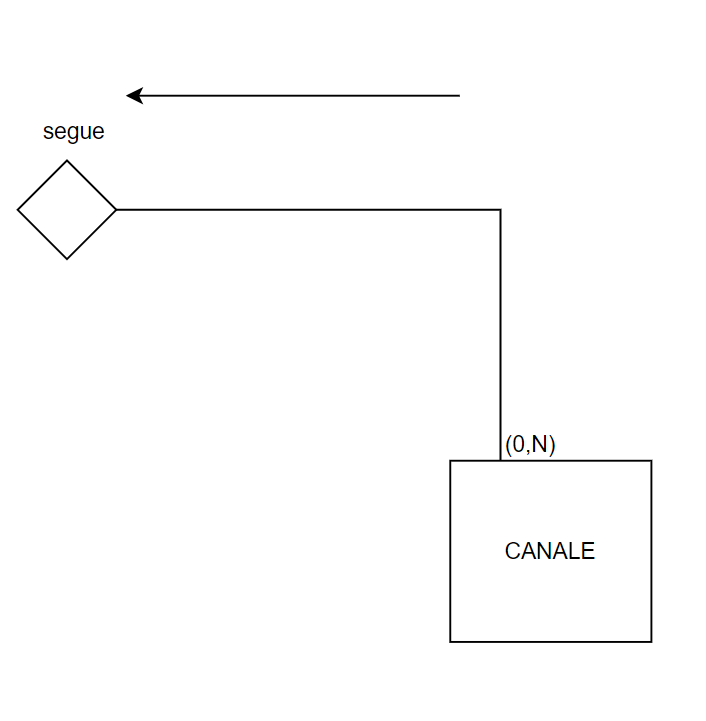
\includegraphics[scale = 0.5]{img/ridondanza111.png}
\end{figure}
\begin{center}
\begin{tabular}{|p{3cm}|p{3cm}|p{3cm}|p{3cm}|}
\hline
\multicolumn{4}{|c|}{\textbf{Tavola degli accessi}}\\
\hline
 \multicolumn{1}{|c|}{\textbf{Concetto}} 
 & \multicolumn{1}{|c|}{\textbf{Costrutto}}
 & \multicolumn{1}{|c|}{\textbf{Accessi}}
 & \multicolumn{1}{|c|}{\textbf{Tipo}}\\
  \hline
  Utente & E & 1 & L\\
  \hline
  Segue & R & 10 & L\\
 \hline
\end{tabular}
\end{center}
Assumendo che, mediamente, un utente segua 10 canali diversi, gli accessi all'associazione sono dati dal seguente calcolo: $(10 \times Volume.Utente) / Volume.Canale = 10$.
\\ \\Analisi dei costi:
\begin{itemize}
    \item Spazio: 0 byte
    \item Tempo:
    \begin{itemize}
        \item Operazione 1: $2 \times (2 \times 958.902)$ accessi in lettura a settimana.
        \item Operazione 2: $10$ accessi in lettura a settimana.
    \end{itemize}
\end{itemize}
Totale: 3.835.618 accessi a settimana.



\newpage
\subsubsection*{Con ridondanza} 
\textbf{Operazione 1:} Un utente inizia a seguire un canale, in media 136.986 volte al giorno.
\begin{figure}[h]
    \centering
    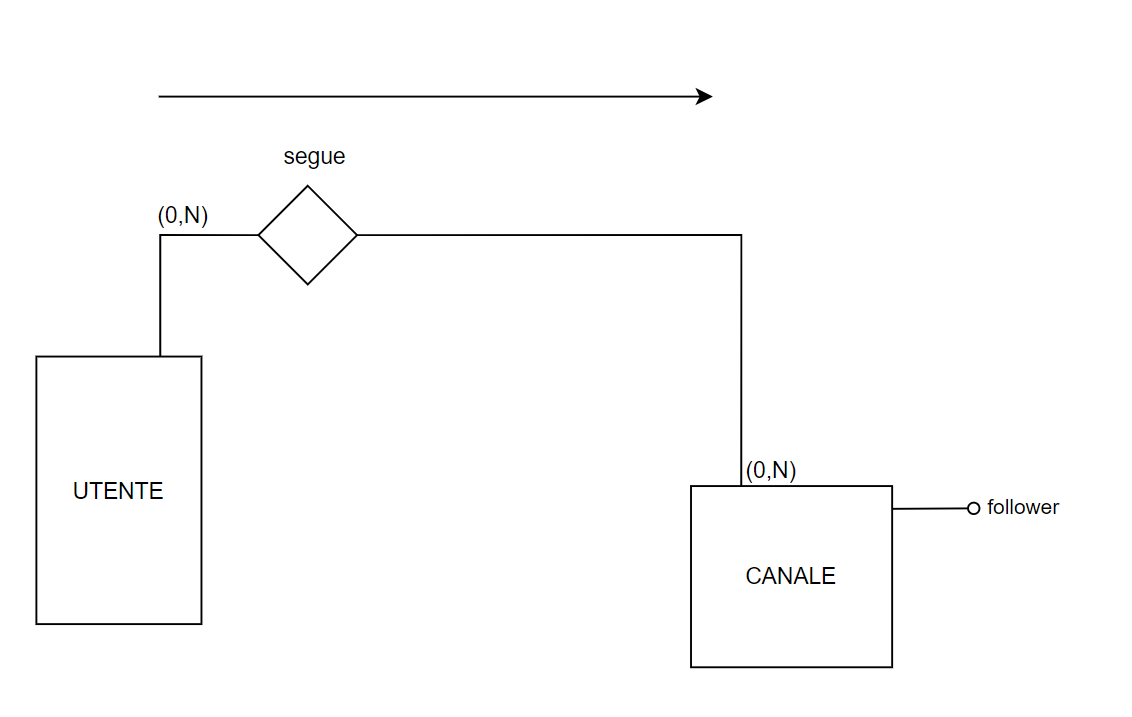
\includegraphics[scale = 0.5]{img/ridondanza2.png}
\end{figure}
\begin{center}
\begin{tabular}{|p{3cm}|p{3cm}|p{3cm}|p{3cm}|}
\hline
\multicolumn{4}{|c|}{\textbf{Tavola degli accessi}}\\
\hline
 \multicolumn{1}{|c|}{\textbf{Concetto}} 
 & \multicolumn{1}{|c|}{\textbf{Costrutto}}
 & \multicolumn{1}{|c|}{\textbf{Accessi}}
 & \multicolumn{1}{|c|}{\textbf{Tipo}}\\
  \hline
  Utente & E & 1 & S\\
  \hline
  Canale & E & 1 & S\\
 \hline
  Segue & R & 1 & S\\
 \hline
\end{tabular}
\end{center}

\textbf{Operazione 2:} Viene calcolata la classifica dei content creator più seguiti (1 volta a settimana).
\begin{figure}[h]
    \centering
    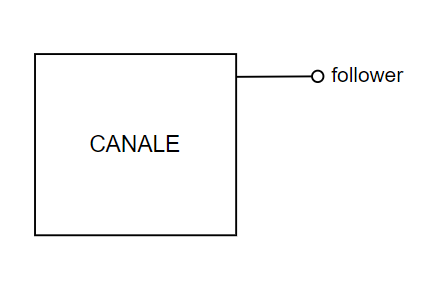
\includegraphics[scale = 0.5]{img/ridondanza22.png}
\end{figure}
\begin{center}
\begin{tabular}{|p{3cm}|p{3cm}|p{3cm}|p{3cm}|}
\hline
\multicolumn{4}{|c|}{\textbf{Tavola degli accessi}}\\
\hline
 \multicolumn{1}{|c|}{\textbf{Concetto}} 
 & \multicolumn{1}{|c|}{\textbf{Costrutto}}
 & \multicolumn{1}{|c|}{\textbf{Accessi}}
 & \multicolumn{1}{|c|}{\textbf{Tipo}}\\
 \hline
  Canale & E & 1 & L\\
 \hline
\end{tabular}
\end{center}
\newpage
Costi:
\begin{itemize}
    \item Spazio: Suppongo di utilizzare 4 byte per il campo \textit{Follower} dell'entità \textit{Canale}, ottengo quindi: 4 byte $\times$ 5.000.000 canali = 20.000.000 byte = 20 MB.
    \item Tempo:
    \begin{itemize}
        \item Operazione 1: $3 \times 958.902$ accessi in scrittura a settimana.
        \item Operazione 2: trascurabile.
    \end{itemize}
\end{itemize}
Totale: 5.753.412 accessi alla settimana

\textbf{Conclusione: } Eliminando la ridondanza diminuisco significativamente non solo il numero di accessi, ma vado anche a risparmiare 20 MB di spazio.








\subsubsection{Eliminazione delle generalizzazioni}
\textbf{Generalizzazione 1:}\\
\begin{figure}[h]
    \centering
    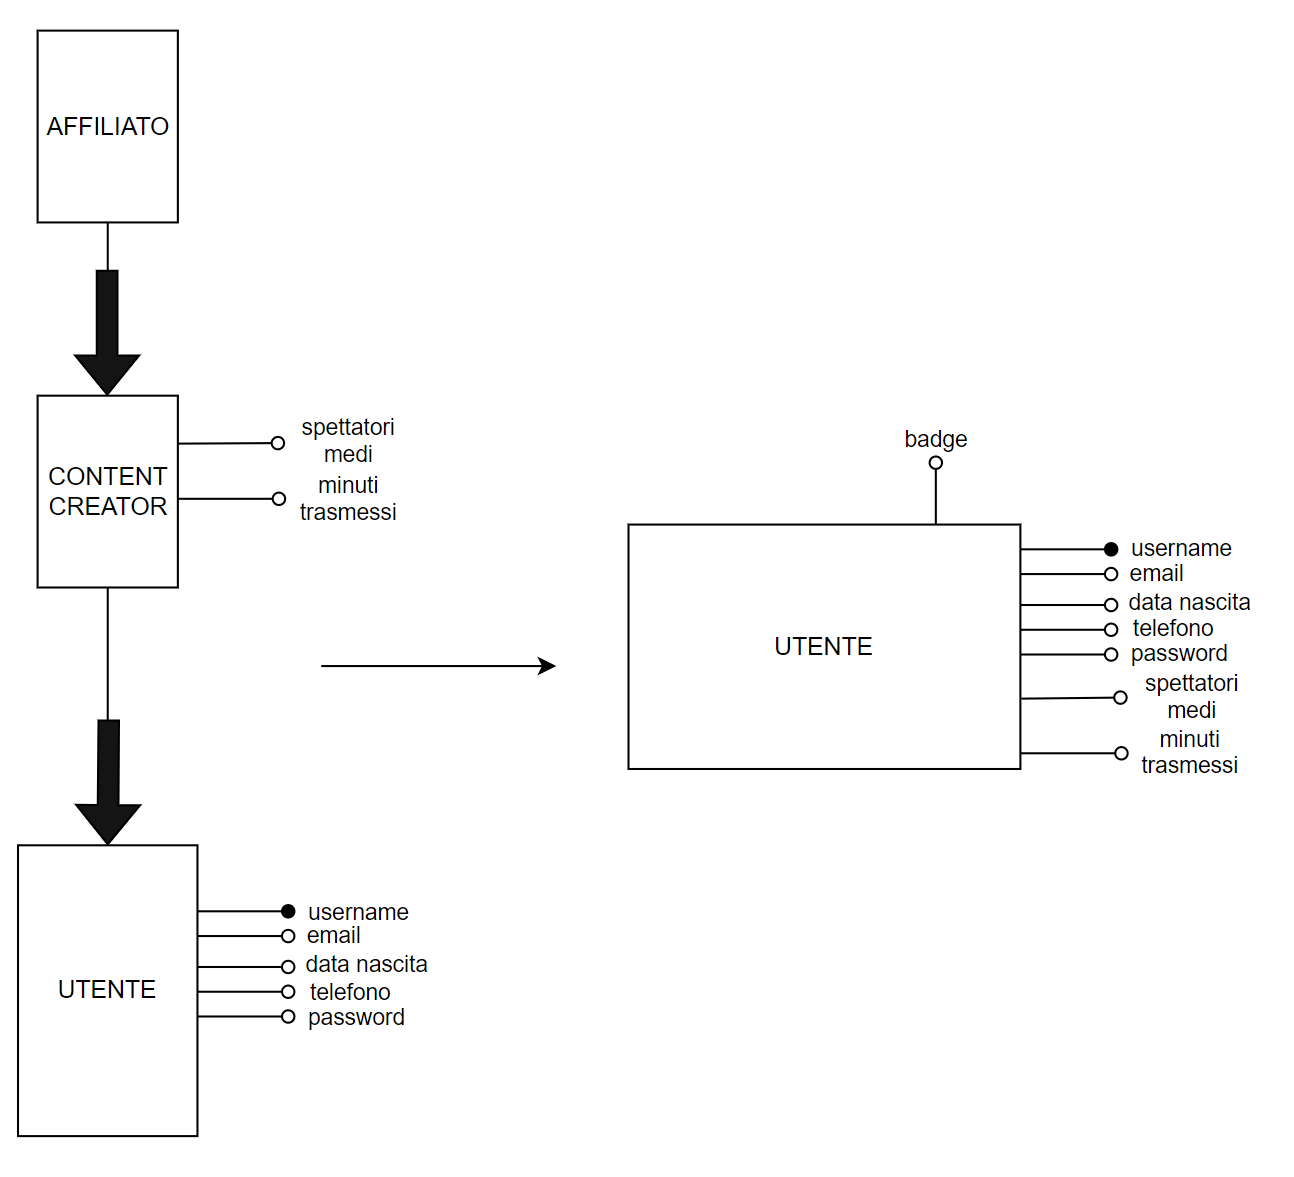
\includegraphics[scale = 0.5]{img/generalizzazione1.png}
\end{figure}\\
\textbf{Business Rules:}
\begin{itemize}
    \item Un \textit{Utente} può diventare \textit{Affiliato} avendo l'attributo booleano \textit{Affiliato} TRUE.
    \item Gli attributi restanti vengono ereditati da \textit{Content Creator} ma possono avere valore 0 nel caso in cui \textit{Utente} decida di non creare alcun contenuto.
\end{itemize}
\textbf{Motivazione:}\\
    L'inclusione delle entità figlie nella loro entità genitore è stata effettuata per ottimizzare lo spazio, mediante la creazione di una nuova tabella che stabilisce una connessione tra \textit{Utente} e \textit{Content Creator}. Questo approccio consente l'ereditarietà degli attributi, come \textit{Minuti trasmessi}, \textit{Spettatori medi} e \textit{Affiliato}, da \textit{Utente}. I primi due sono valori interi e possono rimanere a 0 per gli \textit{Utenti} che non generano contenuti. Nel caso in cui un \textit{Utente}, precedentemente \textit{Content creator}, raggiunga gli obiettivi stabiliti, può acquisire lo status di \textit{Affiliato}. La gestione degli \textit{Affiliati} segue un modello simile su tutte le piattaforme online, consentendo loro di guadagnare un semplice \textit{Affiliato}.


\textbf{Generalizzazione 2:}\\
\begin{figure}[h]
    \centering
    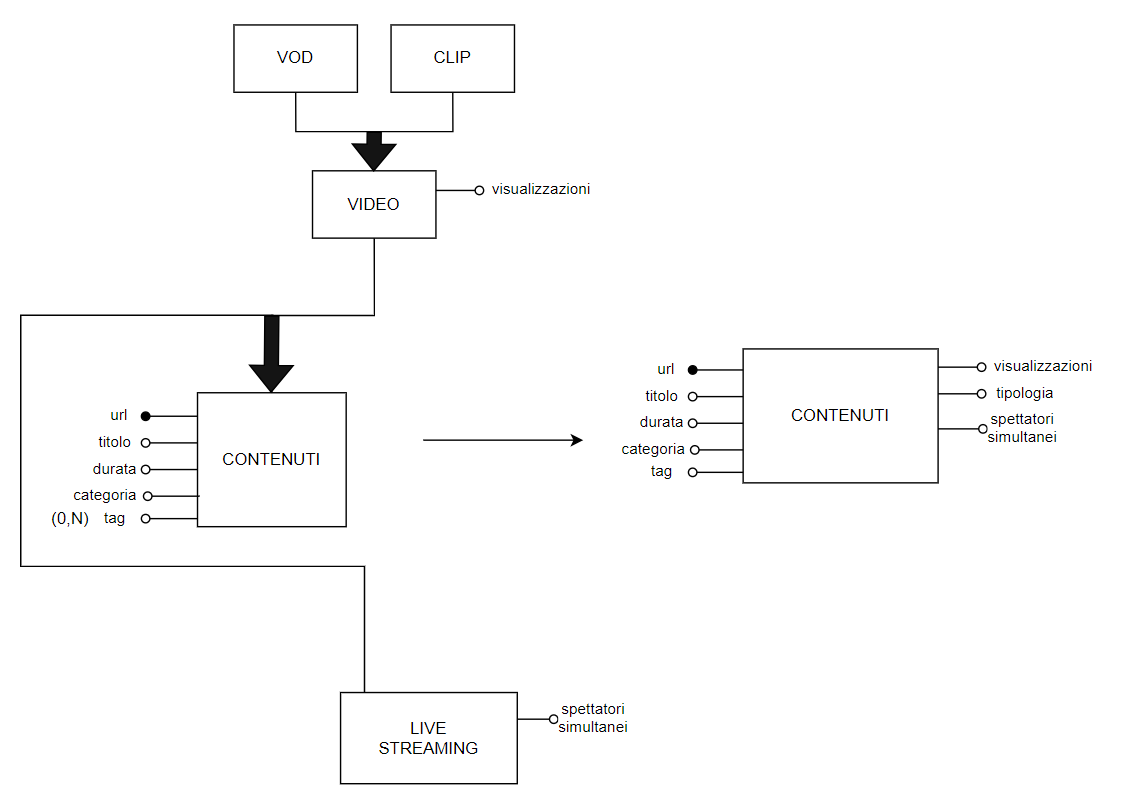
\includegraphics[scale = 0.5]{img/generalizzazione2.png}
\end{figure}\\
\textbf{Business Rules:}
\begin{itemize}
    \item \textit{Tipologia} è un attributo che uso per descrivere le varie istanze delle entità figlie di \textit{Contenuti}.
    \item \textit{Spettatori simultanei} viene utilizzato solamente se \textit{Tipologia} ha valore "Live Streaming".
    \item \textit{Visualizzazioni} viene utilizzato solamente se \textit{Tipologia} ha valore "Video", "Vod" o "Clip".
\end{itemize}
\textbf{Motivazione:}\\
Ho optato per un ulteriore raggruppamento delle entità figlie nella loro entità genitore poiché i \textit{Contenuti} presentano attributi comuni a tutti i figli. Inoltre, considerando che le operazioni non discriminano tra le specializzazioni, la decisione più efficiente è risultata essere l'inclusione dei figli nell'entità genitore. Questa scelta ci ha anche portato a capire che effettuare un raggruppamento del genitore nei figli non sarebbe stata la soluzione ottimale.













\newpage
\subsubsection{Eventuale partizionamento/accorpamento di entità e associazioni}
\textbf{Accorpamento 1:}\\
\begin{figure}[h]
    \centering
    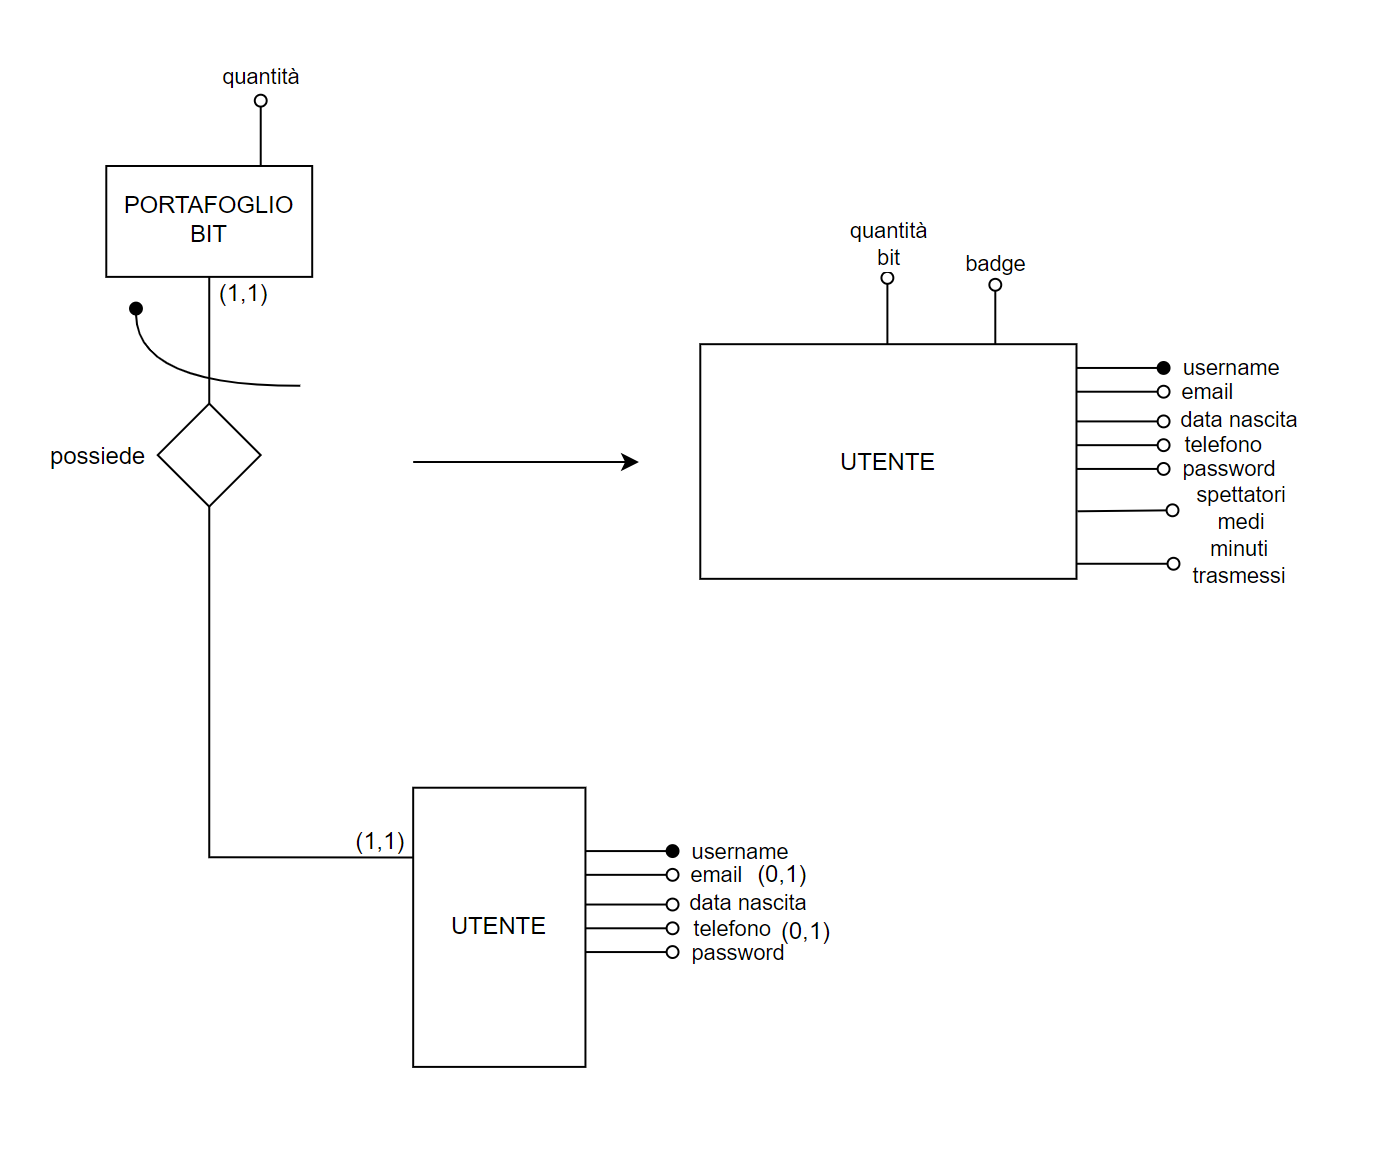
\includegraphics[scale = 0.5]{img/accorpamento1.png}
\end{figure}\\
\textbf{Motivazione:}\\
Ho valutato che le informazioni del \textit{Portafoglio bit} risultano più utili quando sono visualizzate insieme a quelle dell'\textit{Utente}. Considerando il \textit{Portafoglio bit} come un costrutto isolato, offre poche informazioni in quanto richiede sempre lo \textit{Username} per l'accesso. Di conseguenza, poiché ogni \textit{Utente} possiede un unico \textit{Portafoglio bit} e ogni \textit{Portafoglio bit} appartiene a un solo \textit{Utente}, non è necessario creare una nuova tabella per questa entità.



\subsubsection{Eventuale eliminazione delgi attributi composti e degli attributi multivalore}
Gli identificatori principali sono quelli indicati come tali nello schema E-R principale.

\subsubsection{Eventuale scelta degli identificatori principali}
Gli identificatori principali sono quelli indicati come tali nello schema E-R principale.



\newpage
\newgeometry{margin=0.5cm}
\begin{landscape}
\subsection{Schema E-R ristrutturato + business rules}
\vspace{-\parskip} % Elimina lo spazio aggiunto dall'intestazione della subsection
\subsubsection{Schema E-R}
\vspace{-\parskip} % Elimina lo spazio aggiunto dall'intestazione della subsection
\begin{figure}[h]
    \centering
    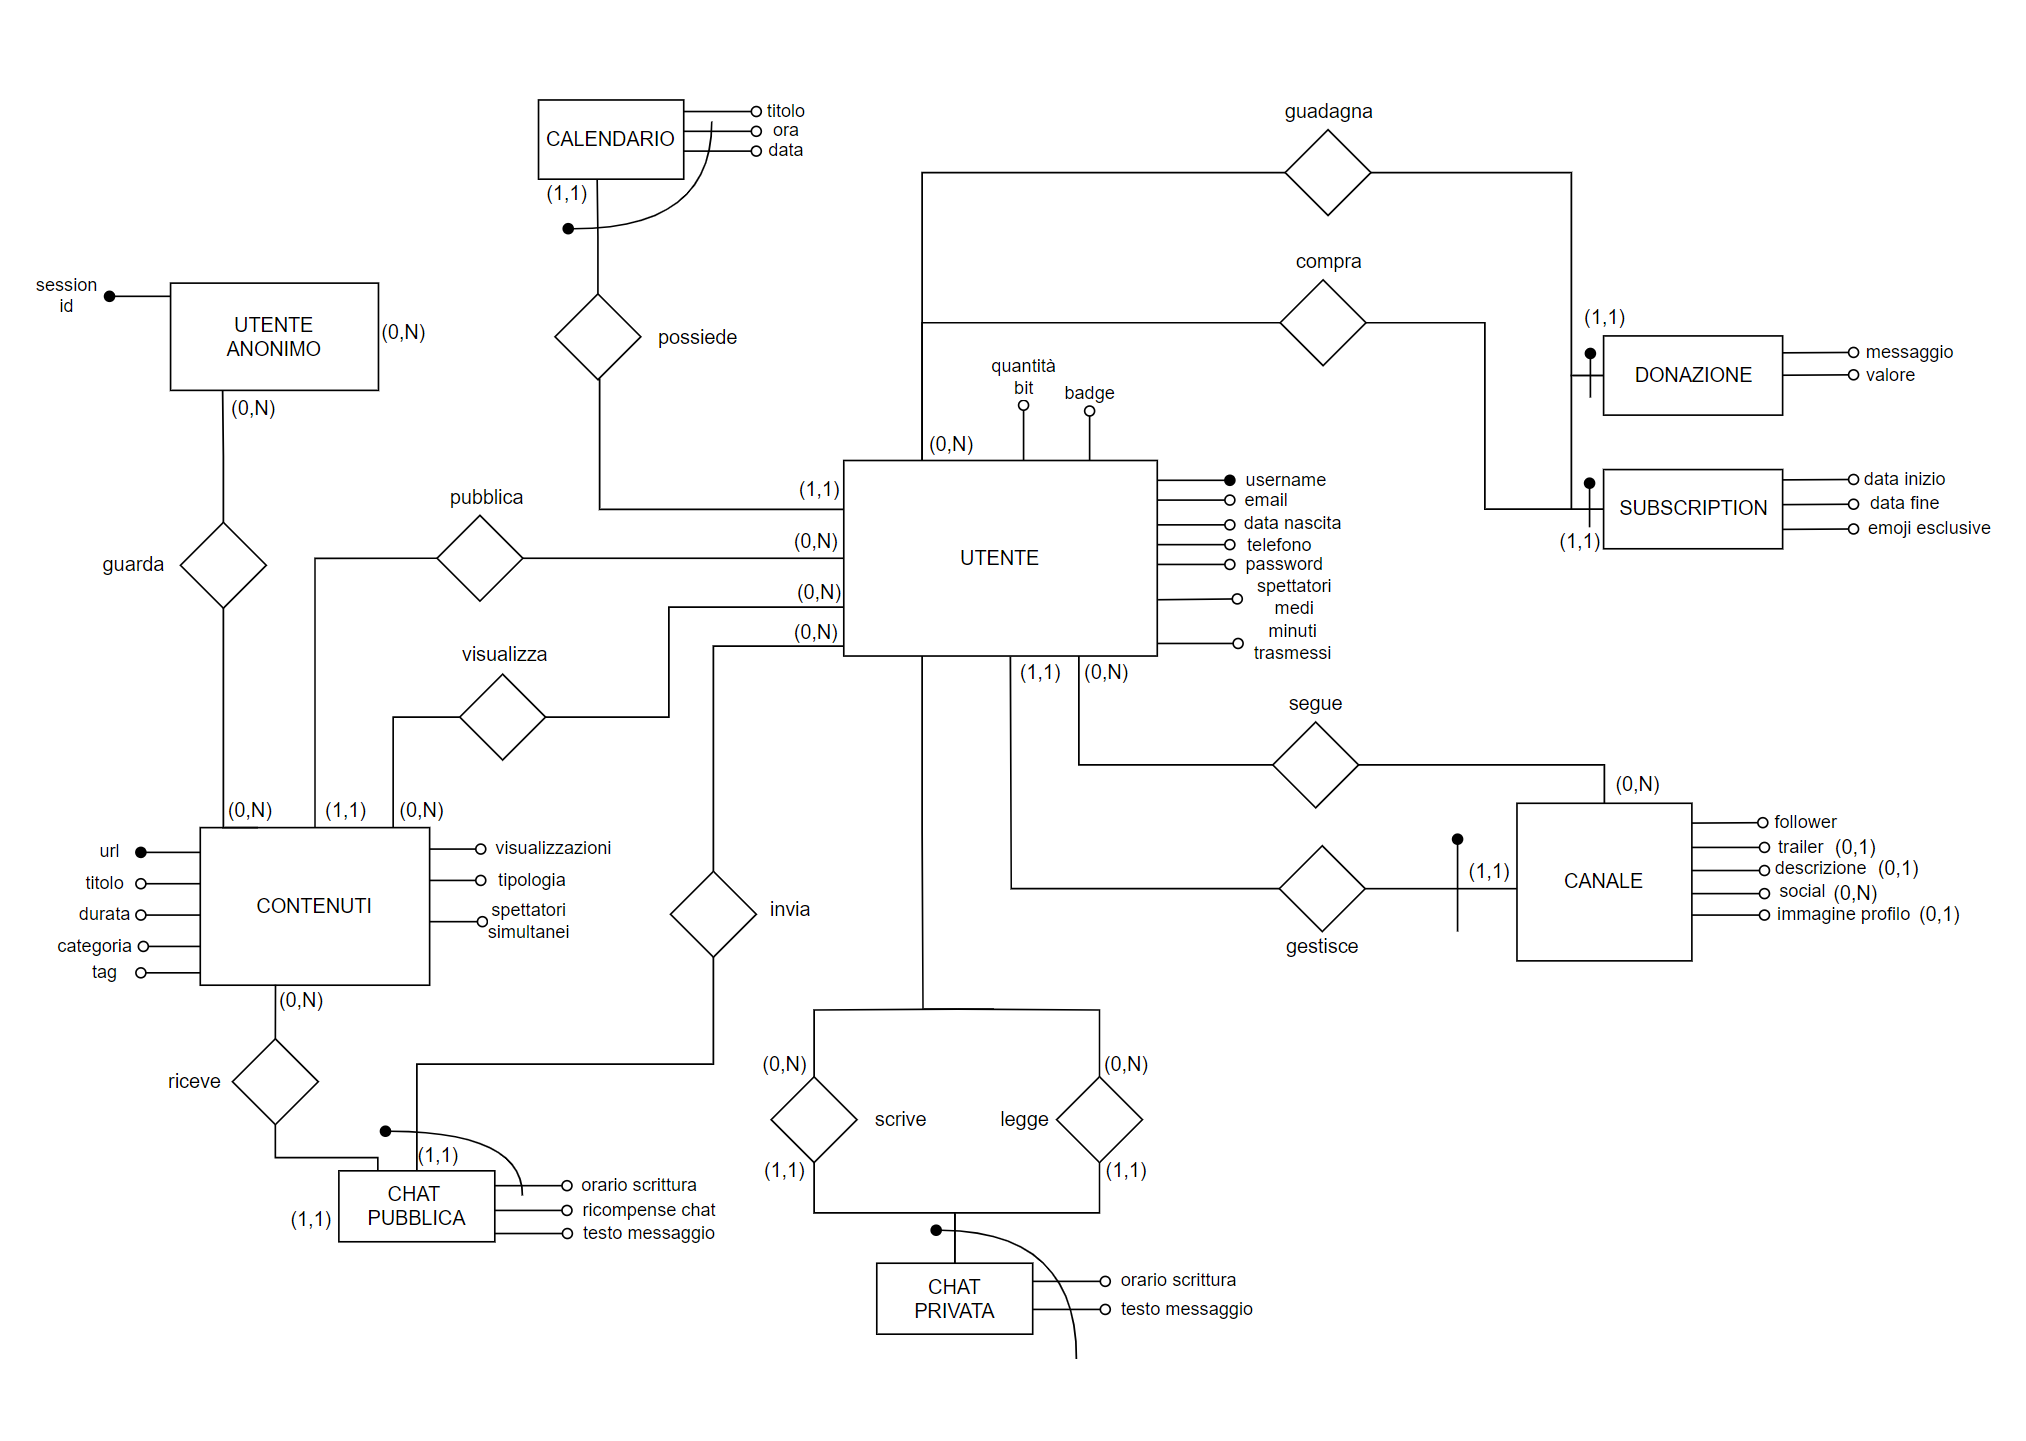
\includegraphics[scale=0.6]{img/ER2.png}
\end{figure}
\end{landscape}
\restoregeometry

%\subsubsection{Business Rules}
%\begin{itemize}
 %   \item Considero gli \textit{Utenti anonimi} come entità separate. Si presume l'esistenza di un algoritmo basato sui log degli utenti non registrati. 
  %  \item Gli \textit{Utenti} devono obbligatoriamente registrarsi sulla piattaforma.
   % \item Gli attributi \textit{Telefono} e \textit{Email} sono stati entrambi impostati come opzionali nello schema E-R poiché per registrarsi alla piattaforma gli utenti devono fornire almeno uno dei due recapiti.
   % \item Il numero di \textit{bit} posseduti da ogni utente deve essere maggiore o uguale a 0.
   % \item Il numero di \textit{bit} donati da un utente a uno streamer deve essere inferiore o uguale al numero di bit posseduti dall'utente in questione.
   % \item I due \textit{Utenti} coinvolti in una\textit{Chat privata} non possono essere lo stesso utente, poiché risulta ovviamente incoerente che un utente invii messaggi a se stesso.
%\end{itemize}










































\subsection{Schema relazionale}
\begin{itemize}
    \item \textbf{Utente} (\underline{username}, email*, telefono*, dataNascita, password, spettatoriMedi, minutiTrasmessi, quantitàBit, affiliato)
    \item \textbf{Calendario} (\underline{username, data, ora}, titolo)
    \item \textbf{UtenteAnonimo} (\underline{sessionId})
    \item \textbf{Contenuti} (\underline{url}, nomeContentCreator, titolo, durata, categoria, tag, visualizzazioni, tipologia, spettatoriSimultanei)
    \item \textbf{ChatPubblica} (\underline{orarioScrittura, utenteMittente, url}, ricompenseChat, testoMessaggio)
    \item \textbf{ChatPrivata} (\underline{orarioScrittura, testoMessaggio, utenteMittente, utenteDestinatario})
    \item \textbf{Canale} (\underline{username}, follower, trailer*, descrizione*, immagineProfilo*, social)
    \item \textbf{Subscription} (\underline{subber, subbed}, dataInizio, dataFine, emojiEsclusive)
    \item \textbf{Donazione} (\underline{donatore, beneficiario}, messaggio, valore)
    \item \textbf{Guarda} (\underline{sessionID, url})
    \item \textbf{Segue} (\underline{seguace}, \underline{seguito})
    \item \textbf{Visualizza} (\underline{url, username})
\end{itemize}

\subsubsection*{Vincoli di integrità referenziale}
\begin{itemize}
  \item \textbf{Calendario} (\textit{username}) referenzia \textbf{Utente} (\textit{username})
  \item \textbf{chatPubblica} (\textit{utenteMittente}) referenzia \textbf{Utente} (\textit{username})
  \item \textbf{chatPubblica} (\textit{url}) referenzia \textbf{Contenuti} (\textit{url}) 
  \item \textbf{chatPrivata} (\textit{utenteMittente}) referenzia \textbf{Utente} (\textit{username})
  \item \textbf{chatPrivata} (\textit{utenteDestinatario}) referenzia \textbf{Utente} (\textit{username})
  \item \textbf{Canale} (\textit{username}) referenzia \textbf{Utente} (\textit{username})
  \item \textbf{Subscription} (\textit{subber}) referenzia \textbf{Utente} (\textit{username})
  \item \textbf{Subscription} (\textit{subbed}) referenzia \textbf{Utente} (\textit{username})
  \item \textbf{Donazione} (\textit{donatore}) referenzia \textbf{Utente} (\textit{username})
  \item \textbf{Donazione} (\textit{beneficiario}) referenzia \textbf{Utente} (\textit{username})
  \item \textbf{Guarda} (\textit{sessionId}) referenzia \textbf{UtenteAnonimo} (\textit{sessionID})
  \item \textbf{Guarda} (\textit{url}) referenzia \textbf{Contenuti} (\textit{url})
  \item \textbf{Segue} (\textit{seguace}) referenzia \textbf{Utente} (\textit{username})
  \item \textbf{Segue} (\textit{seguito}) referenzia \textbf{Utente} (\textit{username})
  \item \textbf{Visualizza} (\textit{url}) referenzia \textbf{Contenuti} (\textit{url})
  \item \textbf{Visualizza} (\textit{username}) referenzia \textbf{Utente} (\textit{username})
\end{itemize}

\newpage
\section{Implementazione}
\subsection{DDL di creazione del database}





\begin{lstlisting}
DROP TABLE IF EXISTS utente CASCADE;
DROP TABLE IF EXISTS utenteAnonimo CASCADE;
DROP TABLE IF EXISTS canale CASCADE;
DROP TABLE IF EXISTS calendario CASCADE;
DROP TABLE IF EXISTS contenuti CASCADE;
DROP TABLE IF EXISTS chatPubblica CASCADE;
DROP TABLE IF EXISTS chatPrivata CASCADE;
DROP TABLE IF EXISTS subscription CASCADE;
DROP TABLE IF EXISTS donazione CASCADE;
DROP TABLE IF EXISTS guarda CASCADE;
DROP TABLE IF EXISTS pubblica CASCADE;
DROP TABLE IF EXISTS segue CASCADE;
DROP TABLE IF EXISTS visualizza CASCADE;

CREATE TABLE utente(
    username varchar PRIMARY KEY,
    email varchar DEFAULT NULL,
    telefono varchar DEFAULT NULL,
    dataNascita date NOT NULL,
    password varchar NOT NULL,
    spettatoriMedi integer DEFAULT 0,
    minutiTrasmessi integer DEFAULT 0,
    quantitaBit integer DEFAULT 0,
    affiliato boolean DEFAULT false
);

CREATE TABLE calendario(
    username varchar,
    data date,
    ora time,
    titolo varchar NOT NULL,
    PRIMARY KEY (username, data, ora)
);

CREATE TABLE utenteAnonimo(
    sessionId varchar PRIMARY KEY
);

CREATE TABLE contenuti(
    url varchar PRIMARY KEY,
    nomeContentCreator varchar NOT NULL,
    titolo varchar NOT NULL,
    durata time NOT NULL,
    categoria varchar NOT NULL,
    tag varchar NOT NULL,
    visualizzazioni integer DEFAULT 0,
    tipologia varchar NOT NULL,
    spettatoriSimultanei integer DEFAULT 0
);

CREATE TABLE chatPubblica(
    orarioScrittura time,
    utenteMittente varchar,
    url varchar,
    ricompenseChat varchar NOT NULL,
    testoMessaggio varchar NOT NULL,
    PRIMARY KEY (orarioScrittura, utenteMittente, url)
);

CREATE TABLE chatPrivata(
    orarioScrittura time,
    testoMessaggio varchar,
    utenteMittente varchar,
    utenteDestinatario varchar,
    PRIMARY KEY (orarioScrittura, testoMessaggio, 
    utenteMittente, utenteDestinatario)
);

CREATE TABLE canale(
    username varchar PRIMARY KEY,
    follower integer DEFAULT 0,
    trailer varchar DEFAULT NULL,
    immagineProfilo varchar DEFAULT NULL,
    social varchar DEFAULT NULL,
    descrizione varchar DEFAULT NULL
);

CREATE TABLE subscription(
    subber varchar,
    subbed varchar,
    dataInizio date DEFAULT NULL,
    dataFine date DEFAULT NULL,
    emojiEsclusive varchar DEFAULT NULL,
    PRIMARY KEY (subber, subbed)
);

CREATE TABLE donazione(
    donatore varchar,
    beneficiario varchar,
    messaggio varchar DEFAULT NULL,
    valore integer DEFAULT 0,
    PRIMARY KEY (donatore, beneficiario)
);

CREATE TABLE guarda(
    sessionID varchar,
    url varchar,
    PRIMARY KEY (sessionID, url)
);

CREATE TABLE segue(
    seguace varchar,
    seguito varchar,
    PRIMARY KEY (seguace, seguito)
);

CREATE TABLE visualizza(
    url varchar,
    username varchar,
    PRIMARY KEY (url, username)
);



ALTER TABLE calendario
ADD FOREIGN KEY (username) REFERENCES utente (username) 
ON DELETE CASCADE ON UPDATE CASCADE;

ALTER TABLE chatPubblica
ADD FOREIGN KEY (utenteMittente) REFERENCES utente (username) 
ON DELETE CASCADE ON UPDATE CASCADE;

ALTER TABLE chatPrivata
ADD FOREIGN KEY (utenteMittente) REFERENCES utente (username) 
ON DELETE CASCADE ON UPDATE CASCADE;

ALTER TABLE chatPrivata
ADD FOREIGN KEY (utenteDestinatario) REFERENCES utente (username) 
ON DELETE CASCADE ON UPDATE CASCADE;

ALTER TABLE canale
ADD FOREIGN KEY (username) REFERENCES utente (username) 
ON DELETE CASCADE ON UPDATE CASCADE;

ALTER TABLE subscription
ADD FOREIGN KEY (subber) REFERENCES utente (username) 
ON DELETE CASCADE ON UPDATE CASCADE;

ALTER TABLE subscription
ADD FOREIGN KEY (subbed) REFERENCES utente (username) 
ON DELETE CASCADE ON UPDATE CASCADE;

ALTER TABLE donazione
ADD FOREIGN KEY (donatore) REFERENCES utente (username) 
ON DELETE CASCADE ON UPDATE CASCADE;

ALTER TABLE donazione
ADD FOREIGN KEY (beneficiario) REFERENCES utente (username) 
ON DELETE CASCADE ON UPDATE CASCADE;

ALTER TABLE guarda
ADD FOREIGN KEY (sessionId) REFERENCES utenteAnonimo (sessionId) 
ON DELETE CASCADE ON UPDATE CASCADE;

ALTER TABLE guarda
ADD FOREIGN KEY (url) REFERENCES contenuti (url) 
ON DELETE CASCADE ON UPDATE CASCADE;

ALTER TABLE segue
ADD FOREIGN KEY (seguace) REFERENCES utente (username) 
ON DELETE CASCADE ON UPDATE CASCADE;

ALTER TABLE segue
ADD FOREIGN KEY (seguito) REFERENCES utente (username) 
ON DELETE CASCADE ON UPDATE CASCADE;

ALTER TABLE visualizza
ADD FOREIGN KEY (url) REFERENCES contenuti (url) 
ON DELETE CASCADE ON UPDATE CASCADE;

ALTER TABLE visualizza
ADD FOREIGN KEY (username) REFERENCES utente (username) 
ON DELETE CASCADE ON UPDATE CASCADE;
\end{lstlisting}












\subsection{DML di popolamento di tutte le tabelle del database}
\begin{lstlisting}
INSERT INTO utente VALUES ('oskar.heise',  'oskar@gmail.com', 
'1234567890', '2002-12-18', 'P4ssw0rd??', 0, 0, 50, false);
INSERT INTO utente VALUES ('mario.rossi', 'mario.rossi@gmail.com',
'9876543210', '1995-05-22', 'M@rioP@ss!', 0, 0, 50, false);
INSERT INTO utente VALUES ('laura.bianchi', 'lauri@yahoo.com',
'7654321098', '1988-11-10', 'L@uraP@ss#', 0, 0, 50, false);
INSERT INTO utente VALUES ('giuseppe.verdi', 'gius.verdi@hotmail.com',
'8765432109', '1980-03-15', 'Giuseppe#123', 0, 0, 50, false);
INSERT INTO utente VALUES ('francesca.rossini', 'fra.ross@gmail.com',
'6543210987', '1992-07-03', 'Fr@ncescaPwd', 0, 0, 50, false);
INSERT INTO utente VALUES ('marco.gallo', 'marco.gallo@gmail.com',
'7890123456', '1985-09-28', 'M@rcoGallo!', 0, 0, 50, false);
INSERT INTO utente VALUES ('anna.ferrari', 'anna.ferrari@yahoo.com',
'8901234567', '1990-01-12', 'AnnaF3rr@ri', 0, 0, 50, false);
INSERT INTO utente VALUES ('luca.martinelli', 'luca.ma@hotmail.com',
'5678901234', '1987-04-08', 'Luca_M@rtin', 0, 0, 50, false);
INSERT INTO utente VALUES ('simona.ricci', 'simona.ricci@gmail.com',
'6789012345', '1983-06-20', 'Sim0naRicci*', 0, 0, 50, false);
INSERT INTO utente VALUES ('paolo.colombo', 'paolo.colo@yahoo.com',
'3456789012', '1998-02-25', 'Pa0loC0lomb0#', 0, 0, 50, false);
INSERT INTO utente VALUES ('roberta.mazza', 'rob.mazza@hotmail.com',
'4567890123', '1982-10-07', 'R0bertaM@zz@', 0, 0, 50, false);
INSERT INTO utente VALUES ('andrea.romano', 'and.roma@gmail.com',
'2345678901', '1993-12-30', 'Andr34R0mano$', 0, 0, 50, false);
INSERT INTO utente VALUES ('elisa.rizzo', 'eli.rizzo@yahoo.com',
'4321098765', '1989-08-18', '3lisaRizz0*', 0, 0, 50, false);
INSERT INTO utente VALUES ('giorgio.conti', 'gio.con@hotmail.com',
'3210987654', '1981-04-05', 'Gi0rgioC0nti!', 0, 0, 50, false);
INSERT INTO utente VALUES ('veronica.santoro', 'vero.sant@gmail.com',
'2109876543', '1996-06-15', 'V3ron!caS@nt0r0', 0, 0, 50, false);
INSERT INTO utente VALUES ('davide.ferri', 'da.fer@yahoo.com',
'1098765432', '1984-09-12', 'D@videF3rri#', 0, 0, 50, false);
INSERT INTO utente VALUES ('sara.lombardi', 'sara.lomba@hotmail.com',
'9012345678', '1991-11-28', 'S@raL0mbardi$', 0, 0, 50, false);
INSERT INTO utente VALUES ('marcello.gatti', 'marce@gmail.com',
'5432109876', '1986-02-14', 'M@rc3ll0G@tti', 0, 0, 50, false);
INSERT INTO utente VALUES ('giulia.palumbo', 'giu.palu@yahoo.com',
'6789012345', '1997-03-08', 'Giuli@P@lumb0', 0, 0, 50, false);
INSERT INTO utente VALUES ('antonio.rocca', 'anto.rocca@hotmail.com',
'1234567890', '1980-07-23', 'Ant0ni0R0cca*', 0, 0, 50, false);
INSERT INTO utente VALUES ('eleonora.damico', 'ele.dami@gmail.com',
'2345678901', '1994-05-18', 'El30n0raD@mico#', 0, 0, 50, false);
INSERT INTO utente VALUES ('marco.ferretti', 'marco.ferre@yahoo.com',
'9876543210', '1987-08-15', 'M@rcoFerr3tti#', 0, 0, 50, false);
INSERT INTO utente VALUES ('silvia.monti', 'silviam@hotmail.com',
'8765432109', '1995-02-02', 'S!lviaM0nti*', 0, 0, 50, false);
INSERT INTO utente VALUES ('andrea.palazzi', 'andr.pala@gmail.com',
'7654321098', '1983-11-20', 'Andr3aP@l@zzi!', 0, 0, 50, false);
INSERT INTO utente VALUES ('valentina.battaglia', 'valenb@yahoo.com',
'6543210987', '1990-04-12', 'V@l3ntinaB#tt@glia', 0, 0, 50, false);
INSERT INTO utente VALUES ('gianni.moretti', 'giannim@gmail.com',
'8901234567', '1982-06-25', 'Gi@nniM0rett!$', 0, 0, 50, false);
INSERT INTO utente VALUES ('francesca.ferri', 'fra.fe@hotmail.com',
'5678901234', '1991-09-18', 'Fr@nc3scaF3rri#', 0, 0, 50, false);
INSERT INTO utente VALUES ('luca.ricci', 'luca.ricci@yahoo.com',
'6789012345', '1988-03-03', 'L#caR1cci*', 0, 0, 50, false);
INSERT INTO utente VALUES ('anna.martini', 'ann.marti@gmail.com',
'3456789012', '1996-07-22', 'AnnaM@rtini123', 0, 0, 50, false);
INSERT INTO utente VALUES ('marco.rossi', 'marco.rossi@hotmail.com',
'4567890123', '1985-12-10', 'M@rcoR0ss!123', 0, 0, 50, false);
INSERT INTO utente VALUES ('elena.galli', 'ele.gal@yahoo.com',
'2345678901', '1993-01-28', '3lenaG@lli#', 0, 0, 50, false);


INSERT INTO utente VALUES ('ninja', 'ninja@gmail.com', '9876543210', 
'1991-06-05', 'N!nj@P@ss123', 2000, 1000, 500, true);
INSERT INTO utente VALUES ('shroud', 'shroud@yahoo.com', '8765432109',
'1994-11-02', 'Shr0ud#987', 1500, 1000, 250, true);
INSERT INTO utente VALUES ('tfue', 'tfue@hotmail.com', '7654321098',
'1997-01-02', 'TfueP@ss!321', 1800, 1200, 400, true);
INSERT INTO utente VALUES ('xqcow', 'xqcow@hotmail.com', '5678901234',
'1996-11-12', 'XqC0wP@ss#', 2500, 1000,  650, true);
INSERT INTO utente VALUES ('lirik', 'lirik@gmail.com', '6789012345',
'1990-10-29', 'L!r!kP@ss456', 800, 1200, 100, false);


INSERT INTO calendario VALUES ('ninja', '2024-11-14', 
'20:00:00', 'NuovaLive');

INSERT INTO utenteAnonimo VALUES ('ajkdsfh7819');
INSERT INTO utenteAnonimo VALUES ('jasdksd1617');

INSERT INTO contenuti VALUES ('www.twitch.tv/videos/1887789454',
'ninja', 'TalkShow', '02:00:12', 'JustChatting', 
'QuattroChiacchiere', 0, 'Live streaming', 1200);
INSERT INTO contenuti VALUES ('www.twitch.tv/videos/1844449454', 
'tfue', 'Gaming', '02:00:12', 'Gaming', 'Giochiamo',
1500, 'VOD', 0);
INSERT INTO contenuti VALUES ('www.twitch.tv/videos/1823349454', 
'tfue', 'Gaming', '00:00:15', 'Gaming', 'Giochiamo',
300, 'clip', 0);

INSERT INTO chatPubblica VALUES ('00:30:23', 'oskar.heise',
'www.twitch.tv/videos/1887789454', 0, 'Buonasera');

INSERT INTO chatPrivata VALUES ('12:30:00', 'ciao!', 'oskar.heise', 
'davide.ferri');
\end{lstlisting}

\begin{lstlisting}
INSERT INTO canale VALUES ('oskar.heise');
INSERT INTO canale VALUES ('mario.rossi');
INSERT INTO canale VALUES ('laura.bianchi');
INSERT INTO canale VALUES ('giuseppe.verdi');
INSERT INTO canale VALUES ('francesca.rossini');
INSERT INTO canale VALUES ('marco.gallo');
INSERT INTO canale VALUES ('anna.ferrari');
INSERT INTO canale VALUES ('luca.martinelli');
INSERT INTO canale VALUES ('simona.ricci');
INSERT INTO canale VALUES ('paolo.colombo');
INSERT INTO canale VALUES ('roberta.mazza');
INSERT INTO canale VALUES ('andrea.romano');
INSERT INTO canale VALUES ('elisa.rizzo');
INSERT INTO canale VALUES ('giorgio.conti');
INSERT INTO canale VALUES ('veronica.santoro');
INSERT INTO canale VALUES ('davide.ferri');
INSERT INTO canale VALUES ('sara.lombardi');
INSERT INTO canale VALUES ('marcello.gatti');
INSERT INTO canale VALUES ('giulia.palumbo');
INSERT INTO canale VALUES ('antonio.rocca');
INSERT INTO canale VALUES ('eleonora.damico');
INSERT INTO canale VALUES ('marco.ferretti');
INSERT INTO canale VALUES ('silvia.monti');
INSERT INTO canale VALUES ('andrea.palazzi');
INSERT INTO canale VALUES ('valentina.battaglia');
INSERT INTO canale VALUES ('gianni.moretti');
INSERT INTO canale VALUES ('francesca.ferri');
INSERT INTO canale VALUES ('luca.ricci');
INSERT INTO canale VALUES ('anna.martini');
INSERT INTO canale VALUES ('marco.rossi');
INSERT INTO canale VALUES ('elena.galli');
INSERT INTO canale VALUES ('ninja');
INSERT INTO canale VALUES ('shroud');
INSERT INTO canale VALUES ('tfue');
INSERT INTO canale VALUES ('xqcow');
INSERT INTO canale VALUES ('lirik');

INSERT INTO subscription VALUES ('oskar.heise', 'ninja', 
CURRENT_TIMESTAMP, CURRENT_TIMESTAMP + INTERVAL '1 month', 4.99);


INSERT INTO donazione VALUES ('oskar.heise', 
'tfue', 'Evvai', 9.99);

INSERT INTO guarda VALUES ('ajkdsfh7819',
'www.twitch.tv/videos/1887789454');

INSERT INTO visualizza VALUES ('www.twitch.tv/videos/1887789454',
'oskar.heise');

INSERT INTO segue VALUES ('oskar.heise',
'ninja');
INSERT INTO segue VALUES ('oskar.heise',
'shroud');
INSERT INTO segue VALUES ('oskar.heise',
'tfue');
INSERT INTO segue VALUES ('oskar.heise',
'lirik');
INSERT INTO segue VALUES ('oskar.heise',
'xqcow');
INSERT INTO segue VALUES ('oskar.heise',
'francesca.ferri');
INSERT INTO segue VALUES ('oskar.heise',
'eleonora.damico');
INSERT INTO segue VALUES ('oskar.heise',
'andrea.palazzi');
INSERT INTO segue VALUES ('oskar.heise',
'giulia.palumbo');
INSERT INTO segue VALUES ('oskar.heise',
'simona.ricci');
\end{lstlisting}
















\subsection{Qualche operazione di cancellazione e modifica per verificare i vincoli e gli effetti causati da operazioni su chiavi esterne}

\begin{lstlisting}
UPDATE utente
SET username = 'ninjaTwitch'
WHERE username = 'ninja';

UPDATE utente
SET username = 'OskarConLaK'
WHERE username = 'oskar.heise';

UPDATE utente
SET quantitaBit = 100
WHERE username = 'OskarConLaK';
\end{lstlisting}




\section{Extra}
\subsection*{Classifica dei content creator più seguiti}
\begin{lstlisting}
SELECT DENSE_RANK() OVER(ORDER BY COUNT(*) DESC) AS Classifica, 
u.username AS username, COUNT(*) as follower
FROM utente u JOIN follower f ON f.follower =  s.username
GROUP BY s.username
LIMIT 25;
\end{lstlisting}



\end{document}